\documentclass{standalone}
\usepackage{tikz}
\usetikzlibrary{3d,arrows, calc, backgrounds, petri, positioning, shadows, shapes}


\tikzset{
	persp/.style={scale=3.0,x={(-0.8cm,-0.4cm)},y={(0.8cm,-0.4cm)}, z={(0cm,1cm)}},
	points/.style={fill=white,draw=black,thick}
	grid/.style={very thin,gray},
	axis/.style={->,ultra thick},
	cube/.style={thick, fill=black!15,opacity=0.5},
	cube hidden/.style={dashed},
	block/.style={
		rectangle, rounded corners,
		draw=black!80,
		fill=black!10, fill opacity=0.5,
		text=black!90, text opacity=1.0,
    text height=1.5ex,
    text depth=.25ex,
    text width=6em,
    text centered
	}
}

\tikzstyle{class}			=[rectangle, rounded corners, draw=black, fill=blue!40, drop shadow, text centered, anchor=north, text=white,    text width=3cm]
\tikzstyle{module}		=[rectangle, rounded corners, draw=black, fill=red!40, 	drop shadow, text centered, anchor=north, text=white,    text width=3cm]
\tikzstyle{component}	=[rectangle, rounded corners, draw=black, fill=green,   drop shadow, text centered, anchor=north, text=black!90, text width=3cm]
\tikzstyle{single}		=[text height=1.5ex, text depth=0.25ex]
\tikzstyle{double}		=[text height=4.0ex, text depth=2.75ex]
\tikzstyle{triple}		=[text height=6.5ex, text depth=5.25ex]
\tikzstyle{quadru}		=[text height=9.0ex, text depth=7.75ex]
\newcommand*{\rootPath}{../}

\begin{document}
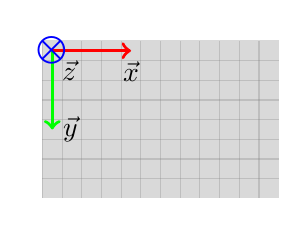
\begin{tikzpicture}
	
	\coordinate	(Ocube)	at (0,0,0);
	\coordinate	(Xcube)	at (1,0,0);
	\coordinate	(Ycube)	at (0,-1,0);
	\coordinate	(Zcube)	at (0,0,-1);
	\coordinate (A) at ($(Ocube)-0.125*(Xcube)-0.125*(Ycube)$);
	\coordinate (B) at ($(Ocube)+2.875*(Xcube)-0.125*(Ycube)$);
	\coordinate (C) at ($(Ocube)-0.125*(Xcube)+1.875*(Ycube)$);
	\coordinate (D) at ($(Ocube)+2.875*(Xcube)+1.875*(Ycube)$);

	\fill[black!50,opacity=0.3] (A)--(B)--(D)--(C)--cycle;
	\foreach \t in {-0.125,+0.125,...,+2.85} { \draw[black!50,opacity=0.3] ($(Ocube)+\t*(Xcube)-0.125*(Ycube)$)--($(Ocube)+\t*(Xcube)+1.875*(Ycube)$); }
	\foreach \t in {-0.125,+0.125,...,+1.85} { \draw[black!50,opacity=0.3] ($(Ocube)-0.125*(Xcube)+\t*(Ycube)$)--($(Ocube)+2.875*(Xcube)+\t*(Ycube)$); }

	\draw[->,very thick,red]		(Ocube)--(Xcube)				node[black,below]				{$\vec x$};
	\draw[->,very thick,green]	(Ocube)--(Ycube)				node[black,right]				{$\vec y$};
	\node[blue]									(Ocube) {$\bigotimes$}	node[black,below right]	{$\vec z$};
\end{tikzpicture}
\end{document}
